% !TEX program = xelatex
\documentclass[compress]{beamer}

\usepackage[english]{babel}
\usepackage{metalogo}
\usepackage{listings}
\usepackage{fontspec}
\usepackage{graphicx}

\usetheme{Nord}

\setsansfont{Andika New Basic}
\setmainfont{Yanone Kaffeesatz}
\setmonofont{Share Tech Mono}

\AtBeginSection[]
{
    \begin{frame}[c,noframenumbering,plain]
        \tableofcontents[sectionstyle=show/hide,subsectionstyle=show/show/hide]
    \end{frame}
}

\AtBeginSubsection[]
{
    \begin{frame}[c, noframenumbering,plain]
        \tableofcontents[sectionstyle=show/hide,subsectionstyle=show/shaded/hide]
    \end{frame}
}

\title{Bijection}
\subtitle{A powerful tool in mathematics}
\author{M Ahsan Al Mahir}
\date{\today}

\begin{document}

\begin{frame}[plain,noframenumbering]
    \maketitle
\end{frame}


\section{Bijection}

\subsection{New way of solving}

\begin{frame}
    \textcolor{NordOrange}{Suppose we want to compute the following sum
    \[{n \choose 0}+{n \choose 1} + \dots  + {n \choose n}\] }
    
    How would you do it?

    \pause \vspace{1em}

    Definitely we wouldn't actually start computing by hand! Because that
    would be \textcolor{NordRed}{REALLY} hard to say the least.
\end{frame}

\begin{frame}
    But we can try to find some values for smaller $n$'s:
    \pause\vspace{1em}

    \[1: {1 \choose 0} + {1 \choose 1} = 2\]\pause
    \[2:\ {2 \choose 0} + {2 \choose 1} + {2 \choose 2} = 4\] \pause
    \[3:\ {3 \choose 0} + {3 \choose 1} + {3 \choose 2} + {3 \choose 3} = 8\] 

    \pause\vspace{1em}

    Do you see any patterns here? Can you guess why?
\end{frame}

\begin{frame}
    Let us start by seeing what these numbers actually mean.
    \textcolor{NordBrightBlue}{We can interpret ${n\choose k}$ as choosing $k$
    items from a box of $n$ balls, for all $k$.} 

    \pause\vspace{1em}

    And ${n \choose 0}+{n \choose 1} + \dots  + {n \choose n}$ means...

    \pause\vspace{1em}
    \begin{center}
        \begin{minipage}{.85\linewidth}
            \textcolor{NordRed}{Choosing some number of balls (any number, $0,
                1, 2, n-1$ or
            $n$) from the set of $n$ balls.}
        \end{minipage}
    \end{center}
    
    \pause \vspace{1em}

    Now the interesting part. How do we actually count it? There are many ways
    to do this, but we will use \textbf{Bijection}.
\end{frame}

\begin{frame}
    \textcolor{NordBrightBlue}{What if we think about selecting a ball as
    labeling it with $1$, and not selecting means marking it with $0$.} 

    \pause\vspace{1em}

    For example, selecting $b_2, b_3, b_5$ from a set of $5$ balls is the same
    is marking them like the following:
    
    \vspace{1em}

    \begin{center}
        \begin{tabular}{ccccc}
            $b_1$ & $b_2$ & $b_3$ & $b_4$ & $b_5$\\
            $0$ & $1$ & $1$ & $0$ & $1$
        \end{tabular}
    \end{center}
\end{frame}

\begin{frame}

    \textcolor{NordRed}{So we have $n$ balls, each labeled with either $1$ or
    $0$, which is just a binary number with lenght $n$   !!}
    
    \vspace{1em}
    And every binary number represents a different set of balls.

    \pause\vspace{1em}

    Can you see why?
\end{frame}

\begin{frame}
    That means the number of ways to select a set of balls is the same as the
    number of binary numbers of length $n$. Which is precisely
    \[\boxed{2^n}\]
    (Because we have two options, $0, 1$, for each of the $n$ positions)
    \pause \vspace{1em}

    And so we have:
    \[{n \choose 0}+{n \choose 1} + \dots  + {n \choose n}=2^n\] 
\end{frame}


\subsection{Defining Bijection}

\begin{frame}

    Just as we said earlier, when we need to count something, we can change our
    interpretation to count something else, that is way easier than the one we
    had to before.\pause
    \vspace{1em}

    That's exactly what bijection does. It gives us a way to turn something
    hard into something easier.

\end{frame}

\begin{frame}
    \texttt{Suppose we have two sets $X, Y$. And for all elements
        of $X$, we can connect it with exactly one element of $Y$. And also for
        all element of $Y$, we can connect it with exactly one element of $X$.
    Then we say that there is a ``bijection'' between $X$ and $Y$.}

    \vspace{1em}
    \begin{figure}
        \begin{center}
            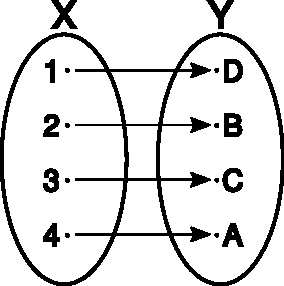
\includegraphics[width=.3\linewidth]{Bijection.pdf}
        \end{center}
    \end{figure}
\end{frame}

\begin{frame}
    And how does that help us?\pause

    \vspace{1em}

    \begin{center}
        \begin{minipage}{.8\linewidth}
            It tells us that the number of elements of $X$ is equal to the number of
            elements of $Y$!!
        \end{minipage}
    \end{center}

    \pause\vspace{1em}

    So if we want to find the number of elements of $X$, then we can
    find a set $Y$ that has a bijection with $X$ and count $Y$ instead!!

    \pause\vspace{1em}

    In our earlier example, we found a bijection between 
    \vspace{1em}

    \begin{center}
        \begin{minipage}{.45\linewidth}
            The number of ways to select a set of balls from a box of $n$ balls
        \end{minipage}\hfill\hspace{.01\linewidth}
        \begin{minipage}{.04\linewidth}
            $\Leftrightarrow$
        \end{minipage}\hfill%
        \begin{minipage}{.45\linewidth}
            The number of binary numbers of length $n$ 
        \end{minipage}
    \end{center}

\end{frame}

\begin{frame}
    Before we jump off to seeing some problems, here is another trivial
    example. \pause
    \vspace{1em}

    Prove that \[{n \choose k} = {n \choose n-k}\] 

    \pause\vspace{1em}

    Ponder for a moment how we would solve this without computation...

    \pause\vspace{1em}

    We solve it by finding a bijection between \texttt{choosing $k$ balls from
    a set of $n$ balls} and \texttt{removing $n-k$ balls from the set of $n$
    balls to be left with $k$ balls}.
\end{frame}


\subsection{Bijection in Action}

\begin{frame}
    Well that's nice, but how do we solve problems with bijection??

    \pause\vspace{1em}

    Let's start by seeing another easy application.
\end{frame}

\begin{frame}
    \textcolor{NordOrange}{
        In how many ways can $n$ be written as sum of
        integers? For example, $3$ can be written in $4$ ways
        \[1 + 1+ 1 = 1+2 = 2 + 1 = 3\] 
    }

    \pause\vspace{1em}

    I will first give you a hint:

    \vspace{1em}

    \begin{center}
        \begin{tabular}{ccccccccccccc}
            ( & 1 & )& +  & ( & 1 & ) &+& ( & 1 & ) & = & 3\\
            ( & 1 & ) &+& ( & 1 & & +& & 1 & ) & = & 3\\
            ( & 1 &  & +& & 1 & ) &+ & ( & 1 & ) & = & 3\\
            ( & 1 &  & +& & 1 &  & +& & 1 & ) & = & 3\\
        \end{tabular}
    \end{center}
\end{frame}


\begin{frame}
    Now we are off to the solution.
    \pause\vspace{1em}

    Consider the $n-1$ spaces between $n$ $1$'s in the following equation:

    \textcolor{NordRed}{
        \[\left(1 \textunderscore\textunderscore 1
                \textunderscore\textunderscore 1 \textunderscore\textunderscore 1
        \dots \textunderscore\textunderscore 1\right) \]
    }

    \pause\vspace{1em}

    If we place \textcolor{NordRed}{$+$} in some of the spaces and
    \textcolor{NordRed}{$) + ($} in the other spaces, then we get a
    ``partition'' like the one we saw before.

    \pause\vspace{1em}
    
    \begin{center}
        \begin{tabular}{ccccccccccccc}
            ( & 1 & )& +  & ( & 1 & ) &+& ( & 1 & ) & = & 3\\
            ( & 1 & ) &+& ( & 1 & & +& & 1 & ) & = & 3\\
            ( & 1 &  & +& & 1 & ) &+ & ( & 1 & ) & = & 3\\
            ( & 1 &  & +& & 1 &  & +& & 1 & ) & = & 3\\
        \end{tabular}
    \end{center}

\end{frame}

\begin{frame}
    Now I assume you can tell me the answer to the question? Write in the chat
    if you've found the answer.

    \pause\vspace{1em}

    \textcolor{NordBrightBlue}{Exactly! The answer is $2^{n-1}$. } 

    \pause\vspace{1em}

    That's because we have $n-1$ places where we can put either $+$ or $)+($,
    so two options.
\end{frame}


\begin{frame}
    Can you explain the bijection here? 

    \pause\vspace{1em}

    Yes, \textcolor{NordBrightBlue}{we found a bijection from the set of ways
    to write $n$ between the set of binary numbers of length $n-1$.} And the
    second set is MUCH easier to compute.
\end{frame}


\begin{frame}

    \textcolor{NordOrange}{
        Ten points are selected on the positive $x$-axis and five points are
        selected on the positive $y$ -axis. The fifty segments connecting the
        ten points on $x$-axis to the five points on $y$-axis are drawn.
        What is the maximum possible number of points of intersection of these
        fifty segments in the interior of the first quadrant?
    }

    \begin{figure}
        \begin{center}
            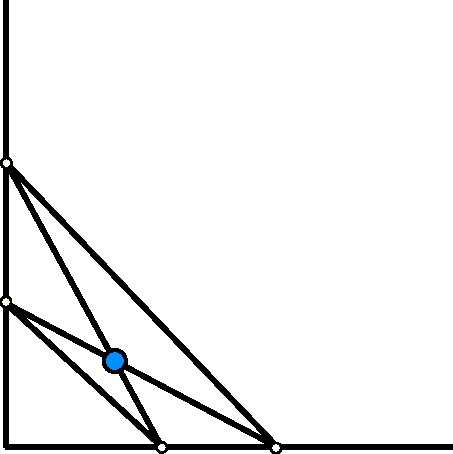
\includegraphics[width=.35\linewidth]{problem_1.pdf}
        \end{center}
    \end{figure}
\end{frame}

\begin{frame}
    The question we have to ask here is, when do two segments intersect? Can
    you answer it?

    \pause\vspace{1em}

    Yes, they intersect whenever \textcolor{NordBrightBlue}{two segments form
    an $\times$.} 

    \pause\vspace{1em}

    No brainer right? But now answer, whend does an $\times$ appear?

    \pause\vspace{1em}

    \textcolor{NordBrightBlue}{An unique cross appears when we select two
    points from the $x$ axis and two points from the $y$ axis.}
\end{frame}

\begin{frame}
    So we have a bijection from the \texttt{number of intersection points} to
    \texttt{the number of crosses} to \texttt{the number of pairs of pairs} from 
    \textcolor{NordRed}{$x$-axis and pairs of points from $y$-axis}.

    \pause\vspace{2em}

    Now we are ready to count the answer. 

    \pause\vspace{2em}

    \textcolor{NordRed}{
        There are a total of ${10 \choose 2}$ ways to select two points from
        $x$-axis. And there are ${5 \choose 2}$ ways to select two points from
        $y$-axis.
    }

    \pause\vspace{1em}

    So the number of ways to select two pairs from the two axes is 
    \[\boxed{{10 \choose 2}{5 \choose 2}}\] 
\end{frame}

\begin{frame}
    So the total number of intersection points is ${10 \choose 2}{5 \choose
    2}$.
\end{frame}


\subsection{One More Problem}

\begin{frame}
    \textcolor{NordOrange}{
        A triangular grid is obtained by tiling
        an equilateral triangle of side length $n$ by $n^{2}$ equilateral
        triangles of side length $1 .$ Determine the number of parallelograms
        bounded by line segments of the grid.
    }

    \begin{figure}
        \begin{center}
            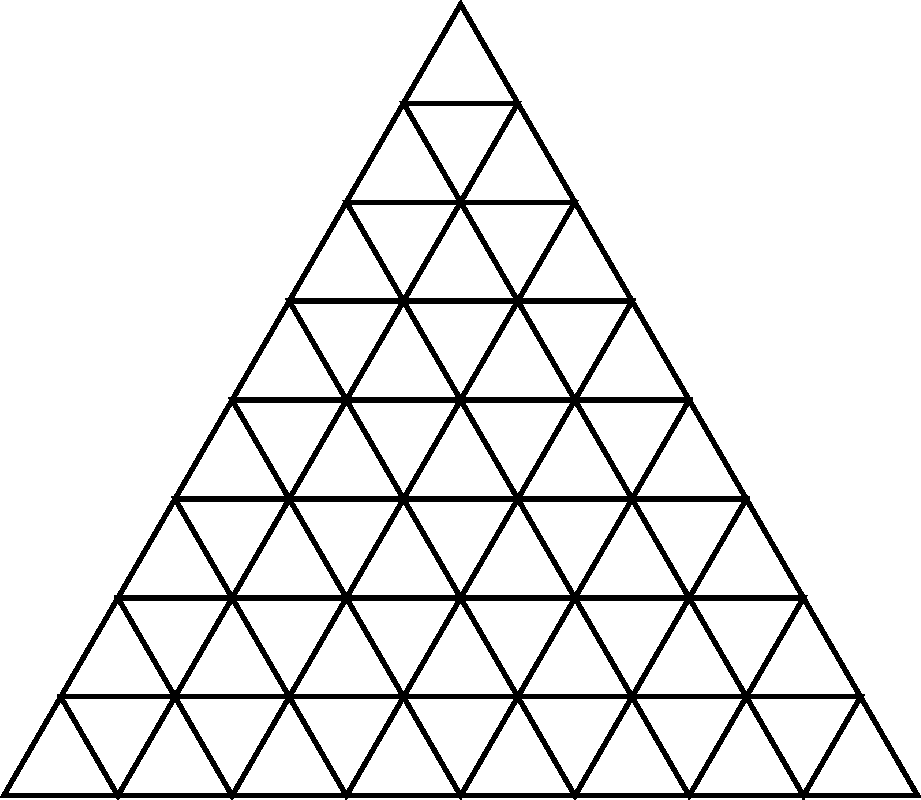
\includegraphics[width=.4\linewidth]{trig_grid_1.pdf}
        \end{center}
    \end{figure}
\end{frame}

\begin{frame}
    First we have to see what the parallelograms might look like:
 
   \begin{figure}
        \begin{center}
            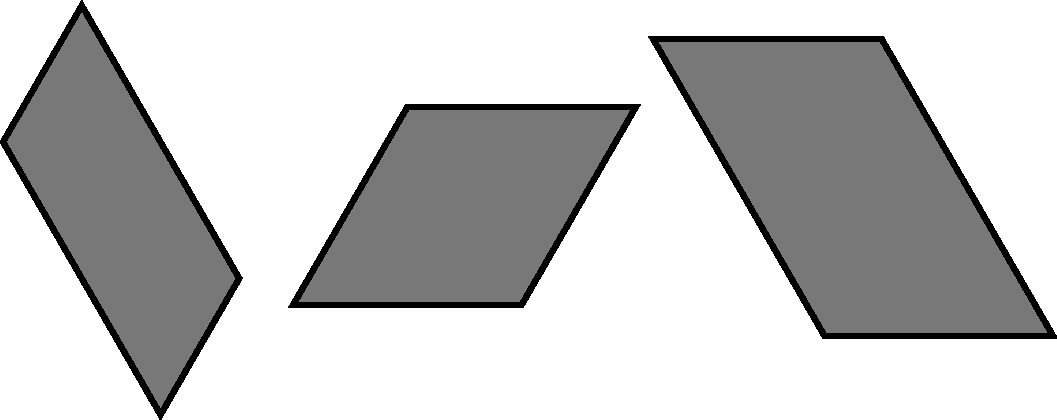
\includegraphics[width=.4\linewidth]{trig_grid_3.pdf}
        \end{center}
    \end{figure}

    \pause\vspace{1em}

    If I told you that there were three different orientations of these
    parallelograms, would you buy it?

    \pause\vspace{1em}

    That's because if you extend those parallelograms' sides, they become
    parallel to two different sides of the triangle. 
\end{frame}


\begin{frame}
    Now what we do is, we work with only one orientation. Because
    \textcolor{NordBrightBlue}{if we can count how many parallelograms there
    are of the first orientation, then we can apply symmetry to count the
    other orientations.}

    \pause\vspace{1em}

    Do you see why?

    \pause\vspace{1em}

    Now, a parallelogram is defined by its parallel sides, right? What if we
    extend those sides?
\end{frame}

\begin{frame}
    If we extend the sides of the parallelogram, and add one more layer at the
    bottom of the grid, we end up with a picture like this

    \pause\vspace{1em}

    \begin{minipage}{.4\linewidth}

        \begin{figure}
            \begin{center}
                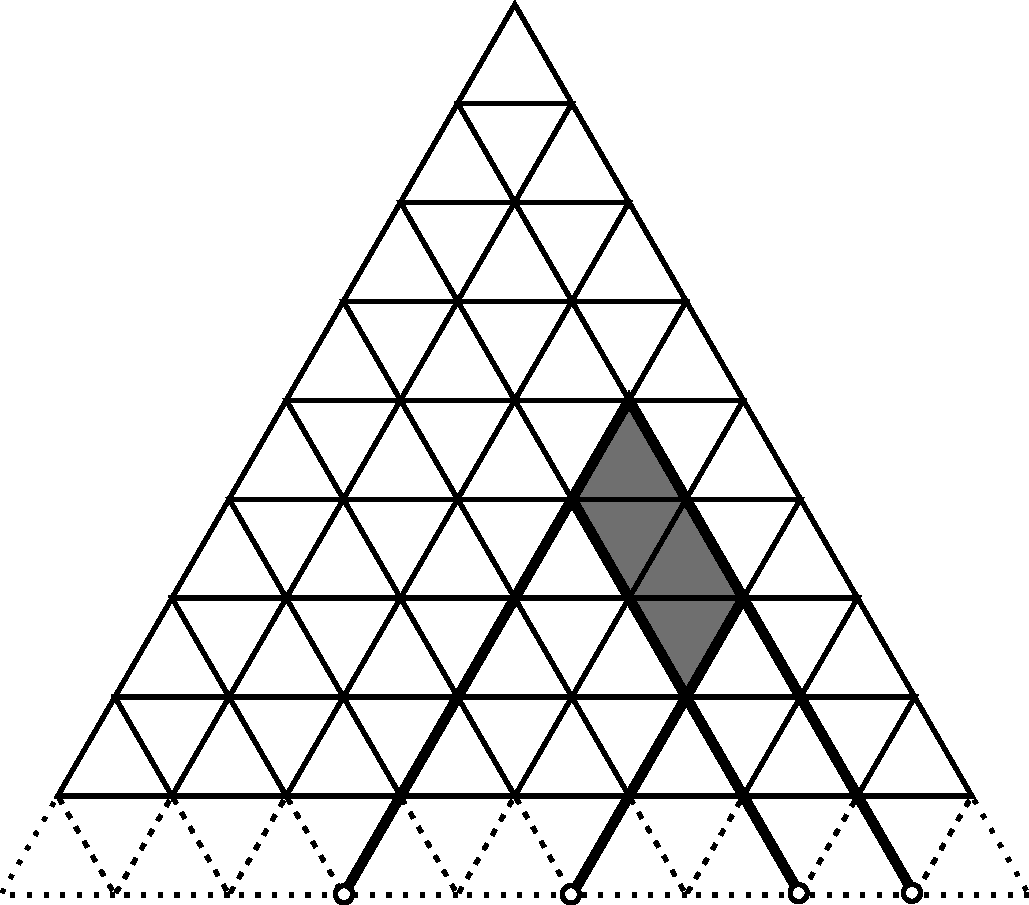
\includegraphics[width=\linewidth]{trig_grid_2.pdf}
            \end{center}
        \end{figure}
    \end{minipage}\hfill%
    \begin{minipage}{.55\linewidth}
        \pause\vspace{1em}

        What's special about this picture?

        \pause\vspace{1em}

        The extended lines intersect the edge in $4$ different points.
        \textcolor{NordRed}{And those $4$ different points define one unique
        parallelogram!}
    \end{minipage}
    
    \pause\vspace{1em}

    \textcolor{NordGreen}{That's a lot to take in, so I will give you 2
    minutes to think about why this happens.}

\end{frame}

\begin{frame}
    As you have seen, $4$ points on the side of the triangle defines one
    parallelogram. 

    \pause\vspace{1em}

    And how many ``quadruple'' of points are there on the extended side?

    \pause\vspace{1em}

    \textcolor{NordRed}{
        \[\boxed{{n+1 \choose 4}}\]
    }

    \pause\vspace{1em}

    So there are a total of ${n+1 \choose 4}$ parallelograms of this
    orientation. 

    \pause\vspace{1em}

    The same goes for the other orientations as well!
\end{frame}

\begin{frame}
    So there are a total of $3\times {n+1 \choose 4}$ parallelograms!

    \pause\vspace{1em}

    Can you explain where we used bijection?

    \pause\vspace{1em}

    Yes \texttt{we used bijection to move from the set of parallelograms to the set of
    quadruples of points on the extended edge}, and it became very easy to
    count.
\end{frame}


\subsection{Conclusion}

\begin{frame}{Further Reader}
    \textcolor{NordOrange}{The Path to Combinatorics for Undergraduate} is a
    really nice boof for cominatorics and Bijection in specific.


    \pause\vspace{1em}

    \textcolor{NordOrange}{Yufei Zhao's Note}
    \url{http://yufeizhao.com/olympiad/bijections.pdf} is a really nice
    resource for bijection related problems.
\end{frame}

\begin{frame}
    In short, \textcolor{NordBrightBlue}{the technique to move from one hard
    to count set to an easy to count set is called Bijection}, it makes your
    life easier.

    \pause\vspace{1em}

    So whenever possible, think about applying bijection to problems
    \textcolor{NordBlack!30!NordWhite}{(after induction though, always apply
    induction at the very beginning)} and see if you can get anything nice :D

    \pause\vspace{1em}

    \textcolor{NordRed}{Happy Problem Solving and Good Luck for TST}

    \textcolor{NordBlack!30!NordWhite}{(you will need it, a lot)}
\end{frame}


\end{document}
